% LCR 阻抗测量与电路辨识 —— Try1–Try3 算法理论（Beamer 学术版）
% 编译：tectonic main.tex  （XeTeX 引擎；中文字体使用系统文泉驿正黑）
\documentclass[UTF8,aspectratio=169,10pt]{ctexbeamer}

\setCJKmainfont{WenQuanYi Zen Hei}[AutoFakeBold=2.2]

\usepackage{amsmath,amssymb}
\usepackage{booktabs}
\usepackage{graphicx}
\graphicspath{{figs/}}

\definecolor{deepblue}{RGB}{15,63,122}
\definecolor{accent}{RGB}{37,99,235}
\definecolor{softblue}{RGB}{239,246,255}
\definecolor{softgray}{RGB}{248,250,252}
\definecolor{okgreen}{RGB}{5,150,105}
\definecolor{warm}{RGB}{161,98,7}

\usefonttheme{professionalfonts}
\setbeamertemplate{navigation symbols}{}
\setbeamersize{text margin left=10pt, text margin right=10pt}
\setbeamercolor{structure}{fg=deepblue}
\setbeamercolor{frametitle}{fg=deepblue}
\setbeamercolor{title}{fg=white}
\setbeamercolor{block title}{fg=white,bg=deepblue}
\setbeamercolor{block body}{bg=softgray,fg=black}
\setbeamercolor{block title example}{fg=white,bg=okgreen}
\setbeamercolor{block body example}{bg=softgray,fg=black}
\setbeamercolor{block title alerted}{fg=white,bg=warm!90!black}
\setbeamercolor{block body alerted}{bg=softgray,fg=black}
\setbeamerfont{frametitle}{size=\large,series=\bfseries}
\setbeamerfont{block title}{size=\small,series=\bfseries}
\setbeamerfont{itemize/enumerate body}{size=\footnotesize}
\setbeamerfont{itemize/enumerate subbody}{size=\scriptsize}
\setbeamertemplate{blocks}[rounded][shadow=false]
\setbeamertemplate{items}[circle]

\setbeamertemplate{frametitle}{%
  \nointerlineskip
  \begin{beamercolorbox}[leftskip=0.4ex,rightskip=0.4ex plus1fil,sep=2pt]{frametitle}
    \usebeamerfont{frametitle}\strut\insertframetitle\strut
  \end{beamercolorbox}%
  {\color{accent}\hrule height 0.9pt}}
\setbeamertemplate{footline}{%
  \hbox to \paperwidth{\hskip2.2ex\scriptsize\color{gray!70!black}LCR Analyzer \;\textperiodcentered\; Try1--Try3 算法理论\hfill
    \color{deepblue}\insertframenumber\,/\,\inserttotalframenumber\hskip2.2ex}%
  \vskip 3pt}

\title{LCR 阻抗测量与电路辨识}
\subtitle{Try1--Try3：统一前向模型、图搜索与参数优化}
\author{LCR Analyzer 项目 \(\cdot\) AlgorithmLcr v4.1.2}
\date{2026 年 9 月}

\begin{document}

% ------------------------------------------------ 1 title
\begin{frame}
  \titlepage
  \begin{center}
    \begin{beamercolorbox}[center,sep=6pt]{block body}
      {\small 给定扫频测量 $Z(f_k)$，寻找电路图 $G$ 与参数 $\theta$，使
      \;$Z_{\mathrm{calc}}(f_k)=b^{\mathsf T}Y^{-1}(f_k)\,b$\; 逼近测量}\\[2pt]
      {\scriptsize 所有拟合图与数字均来自本仓库对四组真实测量数据（10 Hz--10 kHz）的实际运行}
    \end{beamercolorbox}
  \end{center}
\end{frame}

% ------------------------------------------------ 2 problem
\begin{frame}{问题：从黑盒的 $Z(f)$ 恢复电路 $(G,\theta)$}
  \begin{columns}
    \begin{column}{0.55\textwidth}
      \begin{itemize}
        \item 对数扫频得到离散复阻抗 $\{(f_k,Z_k)\}$，$M=20\ldots40$ 点，10 Hz--10 kHz。
        \item 唯一可观测的是\textbf{端口行为} $Z(s)$；结构要靠“假设—计算—比较”的逆问题求解。
      \end{itemize}
      \vspace{0.6ex}
      \begin{block}{三个引擎 = 同一逆问题的三档先验}
        {\footnotesize
        \setlength{\tabcolsep}{3.5pt}
        \begin{tabular}{@{}lll@{}}
          \toprule
          引擎 & 已知 / 未知 & 核心动作\\
          \midrule
          Try1 & 全未知（仅测量） & SP 树枚举 + Foster 辅助\\
          Try2 & 器件已知；接线未知 & 枚举非同构多重图\\
          Try3 & 拓扑·类型已知；数值未知 & 归约 + 多起点拟合\\
          \bottomrule
        \end{tabular}}
      \end{block}
      {\footnotesize 变体：Try2-Tolerance（标称 $\pm$ 容差精调）、内部 Try2.5（宽箱拟合）。}
    \end{column}
    \begin{column}{0.45\textwidth}
      \centering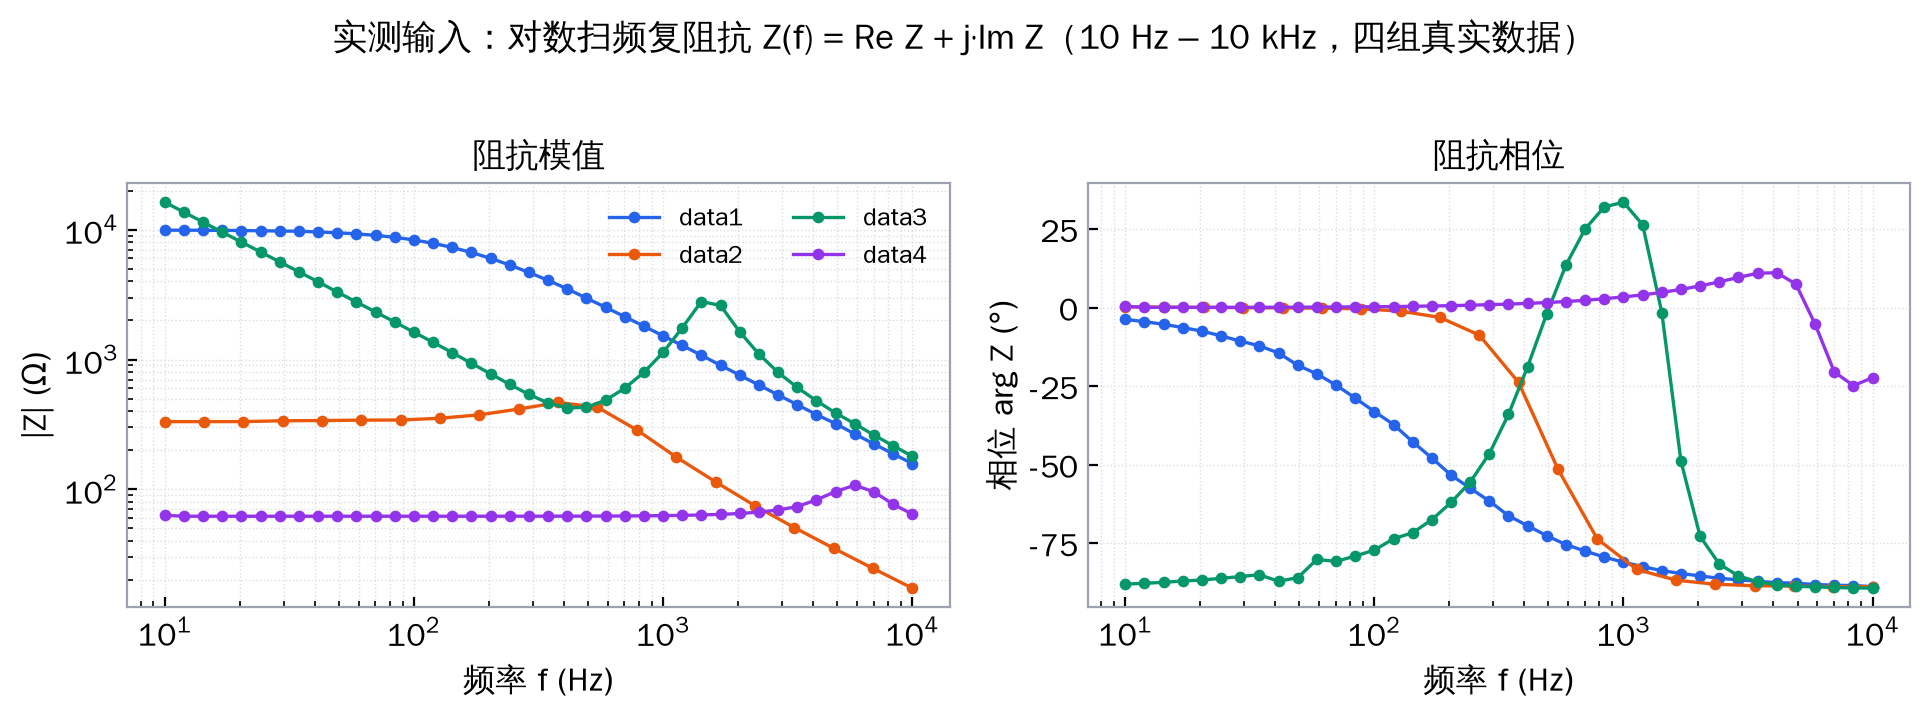
\includegraphics[width=\linewidth]{fig-overview.png}
    \end{column}
  \end{columns}
\end{frame}

% ------------------------------------------------ 3 graph
\begin{frame}{核心抽象：电路 = 多重图}
  \begin{columns}
    \begin{column}{0.53\textwidth}
      \begin{itemize}
        \item \textbf{顶点} = 电气连接点，\textbf{边} = 元件；端口固定为节点 0/1。
        \item 允许\textbf{重边}（同节点对多元件 = 并联），不允许自环；无互感、受控源。
        \item 电感绑定直流电阻：$L{+}R_d$ 是一个器件（最多两个参数），$R_d\ge 0$ 可精确为零。
      \end{itemize}
      \begin{block}{元件模型（$s=j2\pi f$）}
        {\small
        \[
          z_R=R,\qquad z_C=\frac{1}{sC},\qquad z_L=R_d+sL,\qquad y_e=\frac{1}{z_e}
        \]}
      \end{block}
      {\footnotesize 有了这层抽象，“搜索电路结构”= \textbf{搜索图}：Try1/Try2 的离散部分都在图的组合空间上进行。}
    \end{column}
    \begin{column}{0.47\textwidth}
      \centering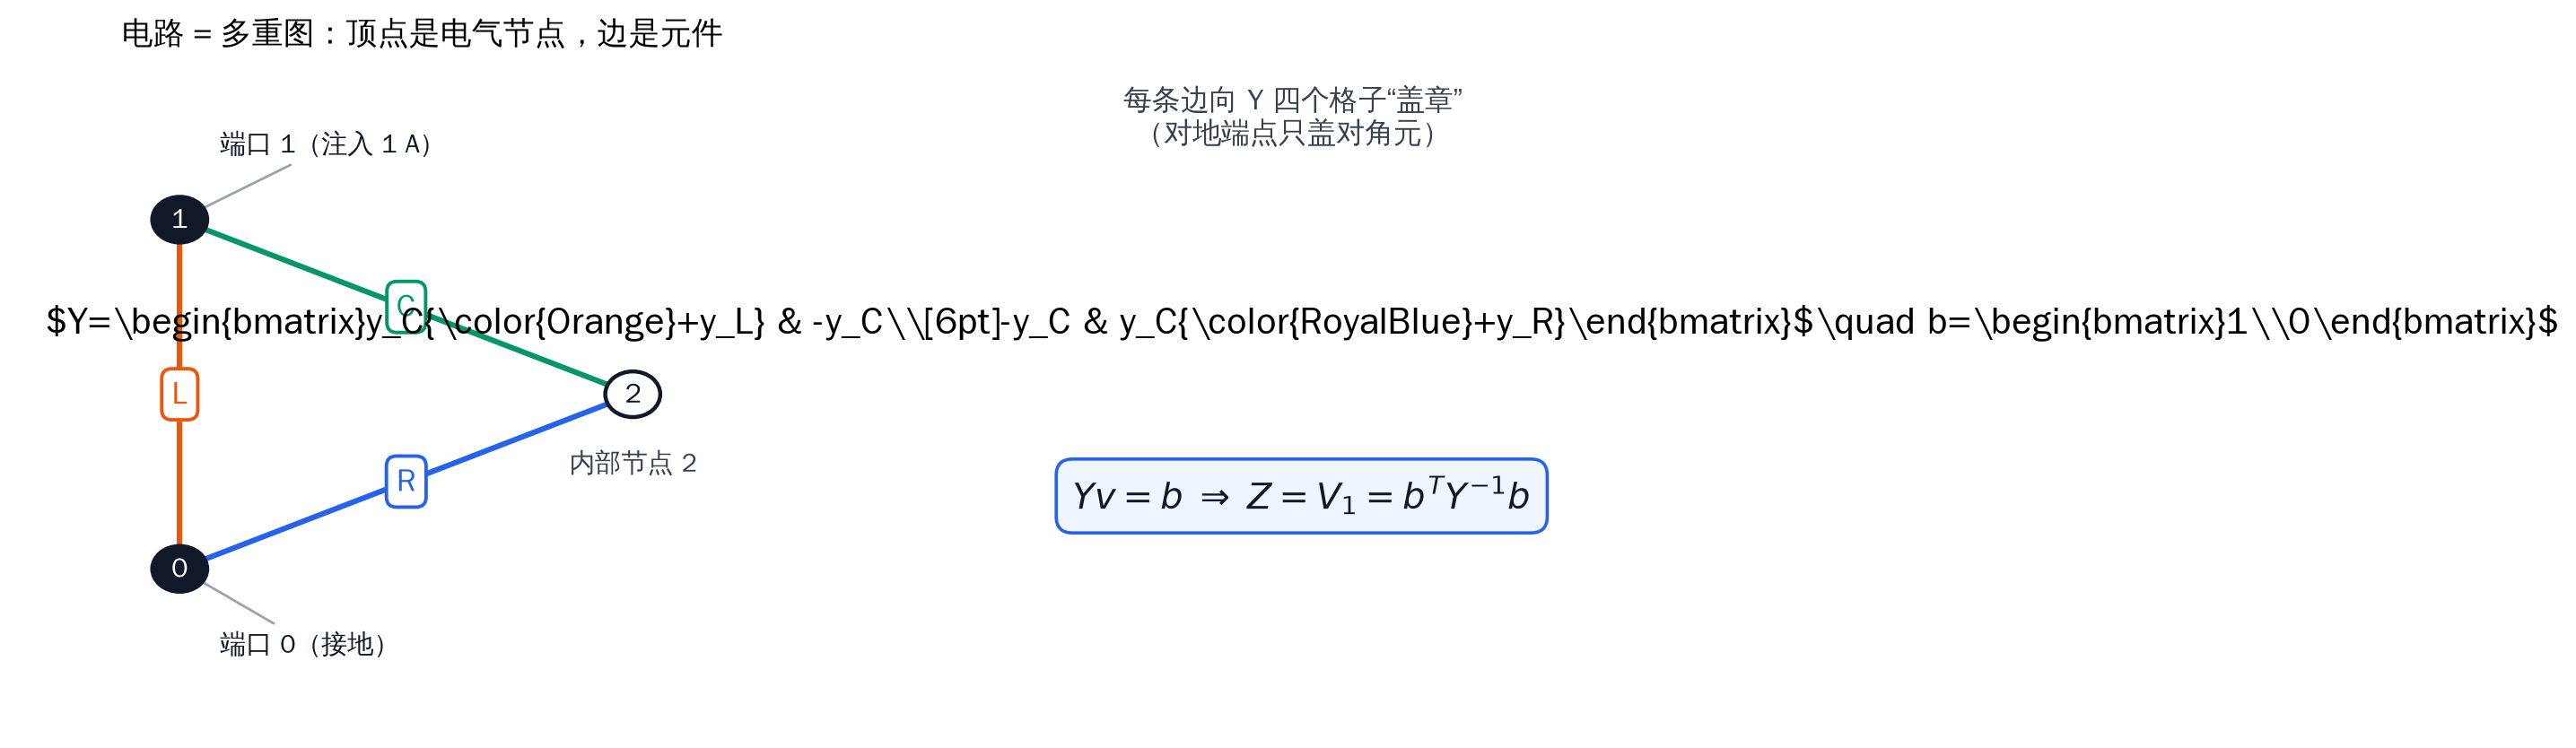
\includegraphics[width=\linewidth]{fig-graph.png}\\
      {\scriptsize 3 节点、3 条边 $L\parallel(R{+}C)$ 与其节点导纳矩阵}
    \end{column}
  \end{columns}
\end{frame}

% ------------------------------------------------ 4 stamp
\begin{frame}{前向模型 I：每条边向 $Y$ “盖一次章”}
  \begin{columns}
    \begin{column}{0.62\textwidth}
      \begin{block}{边的 stamp（导纳 $y$，端点 $u,v$）}
        {\small
        \[
          Y_{uu}\mathrel{+}=y,\qquad Y_{vv}\mathrel{+}=y,\qquad
          Y_{uv}\mathrel{-}=y,\qquad Y_{vu}\mathrel{-}=y
        \]}
      \end{block}
      \begin{itemize}
        \item 地（端口 0）电压恒为 0：\textbf{不进入未知量}，只盖非地端对角元。
        \item 矩阵语言：$Y(s)=\sum_e y_e(s)\,a_e a_e^{\mathsf T}$，$a_e$ 在 $u$ 处 $+1$、$v$ 处 $-1$——\textbf{每加一个元件 = 给 $Y$ 加一个秩 1 矩阵}。
        \item 最小例：节点 1、2 间一条 $R$，$g=1/R$：
              $\;Y=\bigl[\begin{smallmatrix} g & -g\\ -g & g\end{smallmatrix}\bigr]$。
              再复杂的图也只是“多盖几次章”。
      \end{itemize}
    \end{column}
    \begin{column}{0.38\textwidth}
      \begin{block}{为什么用节点导纳矩阵}
        \begin{itemize}
          \item KCL 的直接离散形式，组装\textbf{局部、可加}。
          \item 串并联公式只是它在特殊拓扑下的化简；节点法天然处理\textbf{桥式、重边、任意小图}——Try2 能搜桥式网络的原因。
        \end{itemize}
      \end{block}
    \end{column}
  \end{columns}
\end{frame}

% ------------------------------------------------ 5 Z=b'Y^-1b
\begin{frame}{前向模型 II：端口阻抗 $Z=b^{\mathsf T}Y^{-1}b$}
  \begin{columns}
    \begin{column}{0.62\textwidth}
      \begin{block}{四步推导（单位电流激励）}
        \begin{enumerate}
          \item 端口 0 接地；向端口 1 强制注入 $1\,\mathrm{A}$：$b=e_1$。
          \item KCL 矩阵形式 $Yv=b$，解 $v=Y^{-1}b$。
          \item 因 $I_{\mathrm{port}}=1\,\mathrm{A}$，故 $Z=V_1=b^{\mathsf T}v$：
        \end{enumerate}
        \vspace{-1ex}
        \[
          \boxed{\,Z=b^{\mathsf T}Y^{-1}b\,}
        \]
      \end{block}
      \begin{exampleblock}{手算验证：$R$--$C$ 串联（不用串联公式）}
        {\small $g=1/R,\;y_C=j\omega C$：
        \[
          Y=\begin{bmatrix} g & -g\\ -g & g+y_C\end{bmatrix},\;
          b=\begin{bmatrix}1\\0\end{bmatrix}
          \Rightarrow
          Z=\frac{g+y_C}{g\,y_C}=R+\frac{1}{j\omega C}\;\checkmark
        \]}
      \end{exampleblock}
    \end{column}
    \begin{column}{0.38\textwidth}
      \begin{block}{数值可靠性（\texttt{nodal.cpp}）}
        \begin{itemize}
          \item 最大模缩放 + FullPivLU 求解。
          \item \textbf{有效 rcond}（含装配级 LC 导纳相消；一维矩阵普通条件数恒为 1）与后向误差
                $\rho=\|Yv-b\|/(\|Y\|\|v\|+\|b\|)$。
          \item 状态机 OK / PORT\_OPEN / SINGULAR / ILL\_COND. / NONFINITE——\textbf{不用巨大哨兵值掩盖失败}。
        \end{itemize}
      \end{block}
    \end{column}
  \end{columns}
\end{frame}

% ------------------------------------------------ 6 residual
\begin{frame}{拟合与测量的差距怎么量化：残差、wRMSE 与 AICc}
  \begin{columns}
    \begin{column}{0.62\textwidth}
      \begin{block}{白化相对残差（默认噪声模型）}
        {\small
        \[
          z_{\mathrm{floor}}=\max\!\bigl(10^{-15},\,10^{-9}\,\mathrm{med}|Z_k|\bigr)
        \]
        \[
          r_k=\frac{\bigl[\mathrm{Re}(\hat Z_k-Z_k),\;\mathrm{Im}(\hat Z_k-Z_k)\bigr]^{\mathsf T}}{\max(|Z_k|,\,z_{\mathrm{floor}})}
        \]}
        目标 $J=\sum_k\|r_k\|^2$（相对加权：大/小阻抗同权，近零保护防除零）；
        报告 \textbf{wRMSE}$=\sqrt{\overline{\|r_k\|^2}}$ 与 \textbf{maxRel}；可选逐点协方差 GLS。
      \end{block}
      \begin{block}{复杂度惩罚：AICc（小样本修正）}
        {\small
        \[
          \mathrm{AICc}=n\log\!\bigl(\max(J/n,10^{-300})\bigr)+2k+\frac{2k(k+1)}{n-k-1}
        \]}
        $n=2M$ 个实分量；$k=p+1$（$p$ 个自由参数 + 未知共同方差）。参数越多惩罚越重，防止“多加元件总能更低残差”。
      \end{block}
    \end{column}
    \begin{column}{0.38\textwidth}
      \begin{block}{鲁棒选项（只改拟合权重）}
        \begin{itemize}
          \item Huber IRLS：$2.5\times$中位数阈值降权，$\le 3$ 轮，过半点须为内点。
          \item 原始相对权重的 wRMSE / maxRel \textbf{始终照常报告}。
          \item robust 运行不参与 AICc 校准选择，按 RSS 诊断回退。
        \end{itemize}
      \end{block}
      \vspace{0.8ex}
      \begin{beamercolorbox}[sep=4pt]{block body example}
        指标对所有引擎统一：Try1 做模型选择，Try2 给接线排序，Try3 报告单拓扑拟合质量。
      \end{beamercolorbox}
    \end{column}
  \end{columns}
\end{frame}

% ------------------------------------------------ 7 try3 I
\begin{frame}{Try3（I）：参数化、初值与多起点}
  \begin{columns}
    \begin{column}{0.62\textwidth}
      \begin{block}{优化坐标：让数量级成为“平移”}
        \begin{itemize}
          \item 正参数 R/L/C 用对数坐标 $x=\log_{10}q$（链式因子 $\ln 10\cdot q$）；跨 10 个数量级的搜索变均匀。
          \item DCR 用缩放线性非负坐标 $x=R_d/z_{\mathrm{scale}}$，$z_{\mathrm{scale}}=\max(10^{-9},\mathrm{med}|Z|)$——\textbf{可精确到达 0}（softplus 做不到）。
          \item 显式箱投影：默认 $R\in[10^{-3},10^{7}]\,\Omega$、$L\in[10^{-10},10]\,\mathrm{H}$、$C\in[10^{-13},10^{-3}]\,\mathrm{F}$、$R_d\in[0,10^{7}]\,\Omega$。
        \end{itemize}
      \end{block}
      \begin{block}{物理尺度初值（不靠运气起步）}
        {\small
        \[
          \omega_c=2\pi\sqrt{f_{\min}f_{\max}},\qquad
          R_0=z_{\mathrm{scale}},\quad L_0=\frac{z_{\mathrm{scale}}}{\omega_c},\quad
          C_0=\frac{1}{z_{\mathrm{scale}}\,\omega_c}
        \]
        \vspace{-2.2ex}
        \[
          R_{d,0}=0.1\,z_{\mathrm{scale}}
        \]}
        \vspace{-1ex}

        “中位阻抗 $\times$ 频带几何中心”直接给出各类型元件的正确量级。
      \end{block}
    \end{column}
    \begin{column}{0.38\textwidth}
      \begin{block}{确定性多起点}
        \begin{itemize}
          \item 默认 \textbf{16 起点 $\times$ 160 轮}，种子固定 1——完全可复现。
          \item 起点 0 = 物理尺度初值；其余在对数坐标加 $\pm 2.5$ 个数量级抖动（容差模式在箱内均匀采样）。
          \item DCR 每 4 个起点强制一次 0 初值（零 DCR 是常见真相）。
          \item 取全部起点最优；“收敛到同一解的起点数”（agreeingStarts）本身是诊断量。
        \end{itemize}
      \end{block}
    \end{column}
  \end{columns}
\end{frame}

% ------------------------------------------------ 8 try3 II
\begin{frame}{Try3（II）：解析灵敏度 + Levenberg--Marquardt}
  \begin{columns}
    \begin{column}{0.62\textwidth}
      \begin{block}{解析 Jacobian（对 $Yv=b$ 微分；普通转置，非共轭）}
        {\small
        \[
          \frac{\partial Z}{\partial q_e}=-\frac{\partial y_e}{\partial q_e}\,(V_u-V_v)^{2}
        \]
        \[
          \partial_R y=-R^{-2},\;\;\partial_C y=s,\;\;
          \partial_L y=\tfrac{-s}{(R_d+sL)^2},\;\;\partial_{R_d} y=\tfrac{-1}{(R_d+sL)^2}
        \]}
        直觉：元件两端 $V_u-V_v\approx 0\Rightarrow \partial Z/\partial q\approx 0$——端口“看不见”它（\textbf{可辨识性}的根源）。
      \end{block}
      \begin{block}{阻尼最小二乘步（增广方程，SVD 直接求解）}
        {\small
        \[
          \min_{\Delta}\Bigl\|\begin{bmatrix} J\\ \sqrt{\lambda}\,D\end{bmatrix}\Delta+\begin{bmatrix} r\\ 0\end{bmatrix}\Bigr\|_2,
          \qquad D_{jj}=\max\!\bigl(10^{-8},\|J_{:j}\|\bigr)
        \]}
        JacobiSVD 解增广方程，\textbf{不形成法方程} $J^{\mathsf T}J$（避免条件数平方）；信赖域步长 $\le 2$，越界投影回箱；$\lambda$：初始 $10^{-3}$、成功 $/3$、失败 $\times 10$；终止状态显式输出。
      \end{block}
    \end{column}
    \begin{column}{0.38\textwidth}
      \begin{block}{一轮迭代的闭环}
        \begin{enumerate}
          \item 当前 $x\to$ 组装 $Y(f_k)$
          \item 解 $Yv=b$：$Z$、残差 $r$、Jacobian $J$
          \item SVD 解 LM 步 $\to$ 投影 $\to$ 试探
          \item 更优接受、$\lambda\!/3$；否则 $\lambda\times 10$
        \end{enumerate}
      \end{block}
      \vspace{0.8ex}
      \begin{beamercolorbox}[sep=4pt]{block body}
        病态求值（Reject 级）直接判该起点数值失败，不产出假结果。
      \end{beamercolorbox}
    \end{column}
  \end{columns}
\end{frame}

% ------------------------------------------------ 9 try3 III
\begin{frame}[shrink=8]{Try3（III）：归约流程与可辨识性诊断}
  \begin{columns}
    \begin{column}{0.55\textwidth}
      \begin{block}{拟合前：把“端口看不见的东西”精确归约掉}
        \texttt{R0 死区删除} $\to$ \texttt{精确归约} $\to$ \texttt{域传播} $\to$ \texttt{聚合群上共享拟合}
        \begin{itemize}
          \item 死区：只经一个割点挂接、不含另一端口的子网络对 $Z$ 无贡献（如悬挂三角形）。
          \item 并联 R 倒数和 / 并联 C 求和；串联同类 R/L 相加、C 倒数和；串联 R 折入 DCR；\textbf{不合并并联 L+DCR}。
          \item 归约群允许域按表达式单调传播（两个 $r_{\max}$ 串联可达 $2r_{\max}$）。
        \end{itemize}
      \end{block}
      \begin{block}{拟合后：可辨识性诊断}
        \begin{itemize}
          \item 加权实 Jacobian SVD：秩 / 奇异值 / 条件数——满列秩支持\textbf{局部可辨识}；单点秩亏不证明全局参数族。
          \item 弹性度 $\max_f|q\,\partial Z/\partial q|/|Z|<0.1$ 标 weak；atBound、agreeingStarts 单列；条件满足时给线性化 SE 与 95\% 区间 $C_x=V\,\mathrm{diag}(\sigma_i^{-2})V^{\mathsf T}\cdot\frac{J}{n-p}$。
          \item 分级：IDENTIFIABLE\_LOCAL / AMBIGUOUS\_EQ.\\CLASS / NUMERICALLY\_UNSTABLE / DATA\_INSUFF. / LOCAL\_FIT\_UNCONF.
        \end{itemize}
      \end{block}
    \end{column}
    \begin{column}{0.45\textwidth}
      \centering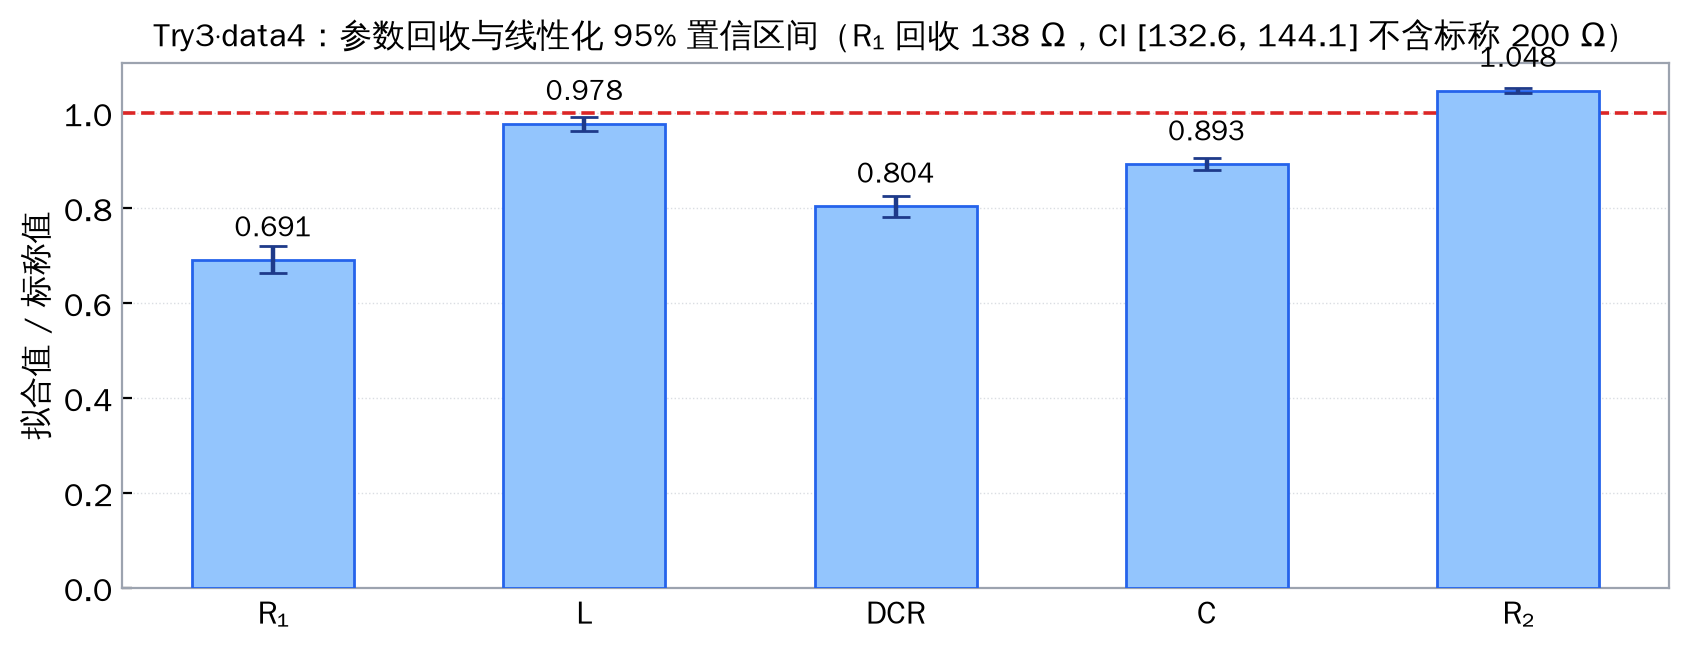
\includegraphics[width=0.86\linewidth]{fig-ident.png}\\
      {\scriptsize data4：rank 5/5、cond 32.8、9/16 起点一致——局部可辨识；但 $R_1$ 回收 138 Ω，CI [132.6, 144.1] \textbf{不含标称 200 Ω}：槽路阻尼由 $R_1$ 与 DCR 强相关地共同提供。}
    \end{column}
  \end{columns}
\end{frame}

% ------------------------------------------------ 10 try2 I
\begin{frame}{Try2（I）：图怎么搜——有限空间的完整枚举}
  \begin{columns}
    \begin{column}{0.55\textwidth}
      \begin{block}{节点数范围与槽位多重集}
        \[
          \text{连通且含两端口}\;\Longleftrightarrow\;2\le V\le E+1
        \]
        \begin{itemize}
          \item 连通图至少 $V-1$ 条边；端口本身占 2 个节点。
          \item 固定 $V$：$\tbinom{V}{2}$ 个\textbf{节点对槽位}，$E$ 条边 = 大小为 $E$ 的多重集（$V{=}3$：$m_{01}+m_{02}+m_{12}=E$）。
          \item DFS 允许重复取同一槽 $\to$ \textbf{天然支持并联重边}；禁止自环。
        \end{itemize}
      \end{block}
      \begin{block}{规范化去重（canonicalization）}
        \begin{itemize}
          \item 结构过滤：无孤立节点；\textbf{活动性}（全部元件端口连通，完整割点死区排除）。
          \item 内部节点重命名与互易端口交换不改变电路 $\to$ 枚举置换、取\textbf{字典序最小签名}去重。
          \item 器件赋值：跳过相同器件的重复排列，带值图再规范化去重。
          \item 支持 $E\le 8$，含桥式与重边；组合数随 $E$ 急增。
        \end{itemize}
      \end{block}
    \end{column}
    \begin{column}{0.45\textwidth}
      \centering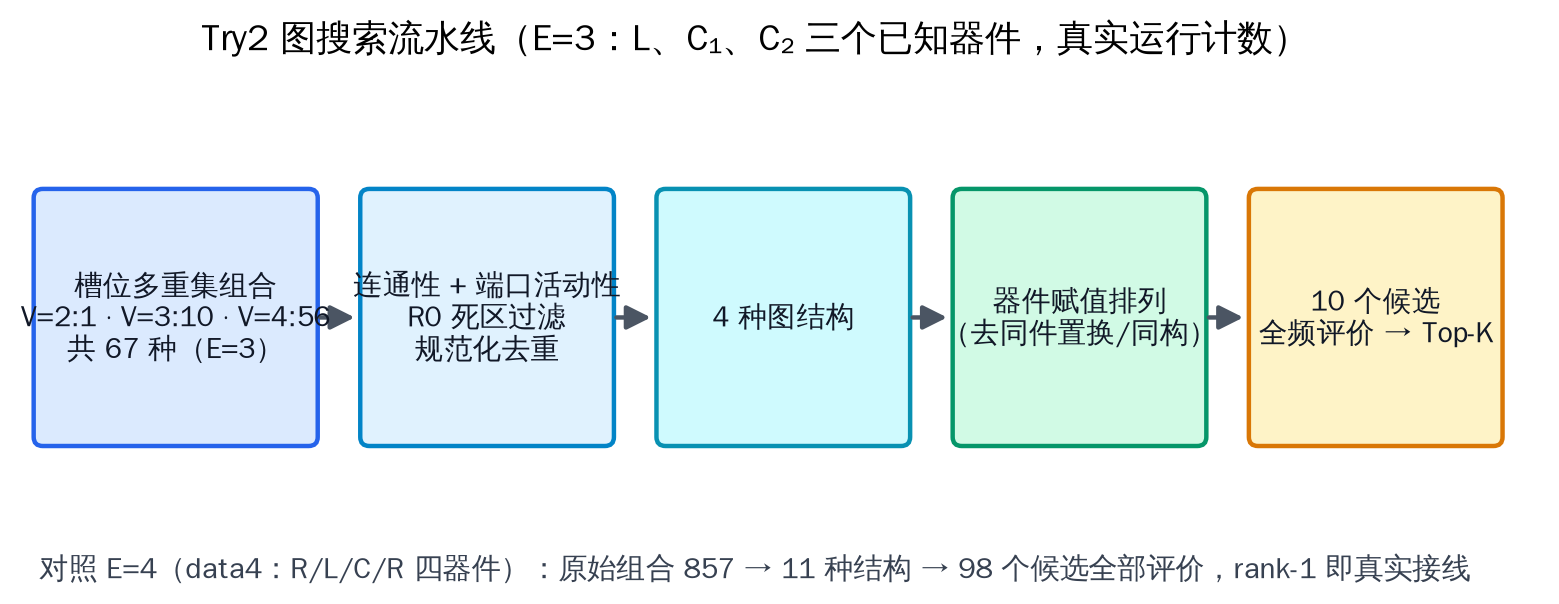
\includegraphics[width=\linewidth]{fig-funnel.png}
    \end{column}
  \end{columns}
\end{frame}

% ------------------------------------------------ 11 try2 II
\begin{frame}[shrink=8]{Try2（II）：评价、排序与实测验证}
  \begin{columns}
    \begin{column}{0.42\textwidth}
      \begin{block}{Exact 模式（默认）：固定参数，只比接线}
        \begin{itemize}
          \item 每个候选图在\textbf{全部频点}前向求值（0 自由参数），按共同 RSS 排序。
          \item Top-K：观测频点数值等价（默认 $10^{-6}$）聚类出代表元。
          \item \textbf{条件最优证书}：枚举完整 $+$ 无数值失败 $\Leftrightarrow$ 可声明该有限空间全局最优；连续拟合永远只是局部方法。
        \end{itemize}
      \end{block}
      \begin{block}{Tolerance 模式}
        显式百分比容差才启用；每元件保持物理身份与自己的容差箱；标称零 DCR 无绝对容差则\textbf{固定为零}。
      \end{block}
      \begin{exampleblock}{实测 data4（R/L/C/R）}
        857 种组合 $\to$ 11 种结构 $\to$ \textbf{98 个候选全部评价，rank-1 恰为真实接线}；标称值 wRMSE 5.26\%，数值拟合后 0.50\%。
      \end{exampleblock}
    \end{column}
    \begin{column}{0.58\textwidth}
      \centering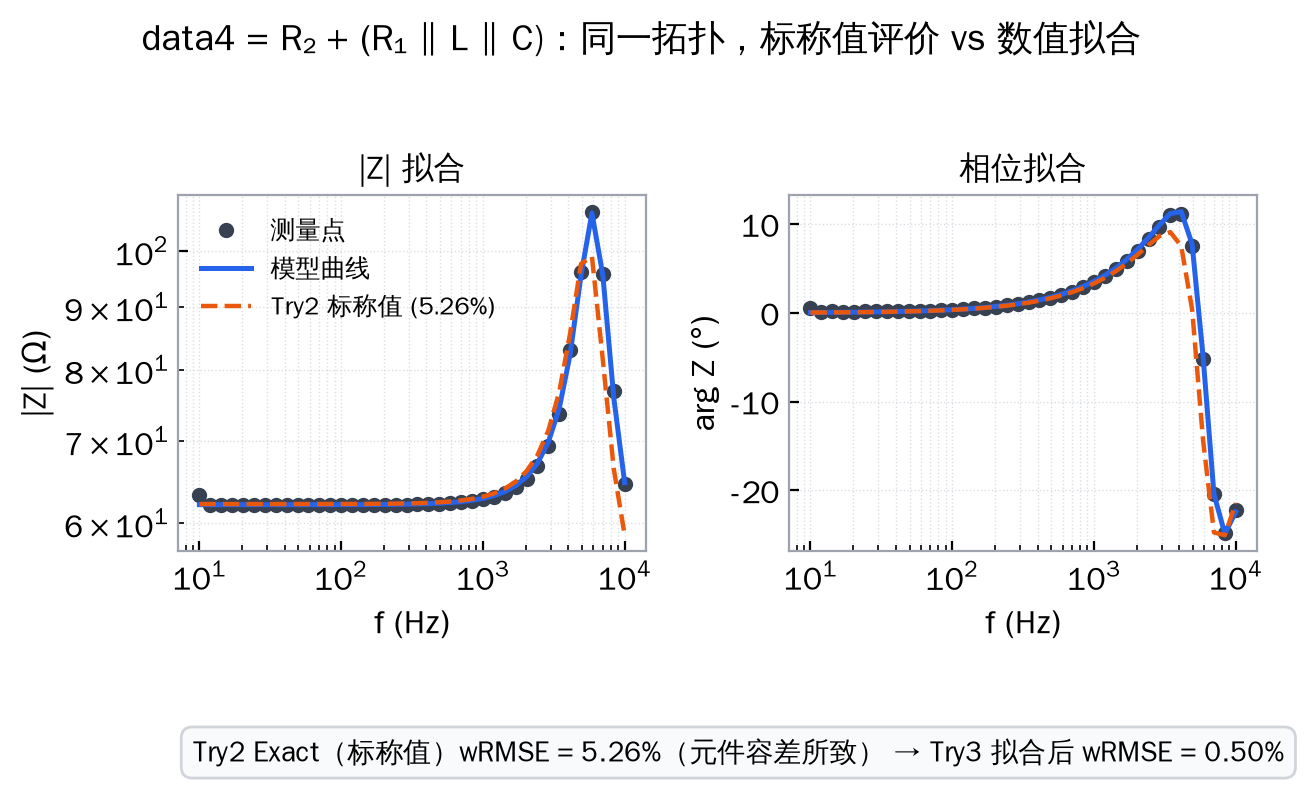
\includegraphics[width=0.88\linewidth]{try3-data4-4.png}
    \end{column}
  \end{columns}
\end{frame}

% ------------------------------------------------ 12 try1 I
\begin{frame}{Try1（I）：规范串并联（SP）树的枚举}
  \begin{columns}
    \begin{column}{0.55\textwidth}
      \begin{block}{假设空间：SP 表达式树}
        叶子 = 器件 R / C / L(+DCR)；内部节点仅 SER 与 PAR。逐层递归构造（器件数拆分 + 交替运算、子树类型 $\ne$ 父节点、深度 $\le$ maxDepth）：
        \[
          Z_S=\sum_i Z_i,\qquad Z_P=\Bigl(\sum_i \frac{1}{Z_i}\Bigr)^{-1}
        \]
      \end{block}
      \begin{block}{规范化规则：同一电路只留一棵树}
        \begin{itemize}
          \item 同运算扁平化 $S(S(a,b),c)\to S(a,b,c)$；子树按键排序。
          \item 不生成可直接归约的结构：SER 下同类叶（$R{+}R$、$C{+}C$、$L{+}L$）、SER 下 $R{+}L$（折入 DCR）；PAR 下同类 R/C 不生成，但\textbf{保留并联 L}。
          \item 默认 maxN=4、maxDepth=4：\textbf{130 棵规范树}（n=1..4，真实运行计数）。
          \item 器件数 = \textbf{规范不可约等效模型}器件数，非物理封装数。
        \end{itemize}
      \end{block}
    \end{column}
    \begin{column}{0.45\textwidth}
      \centering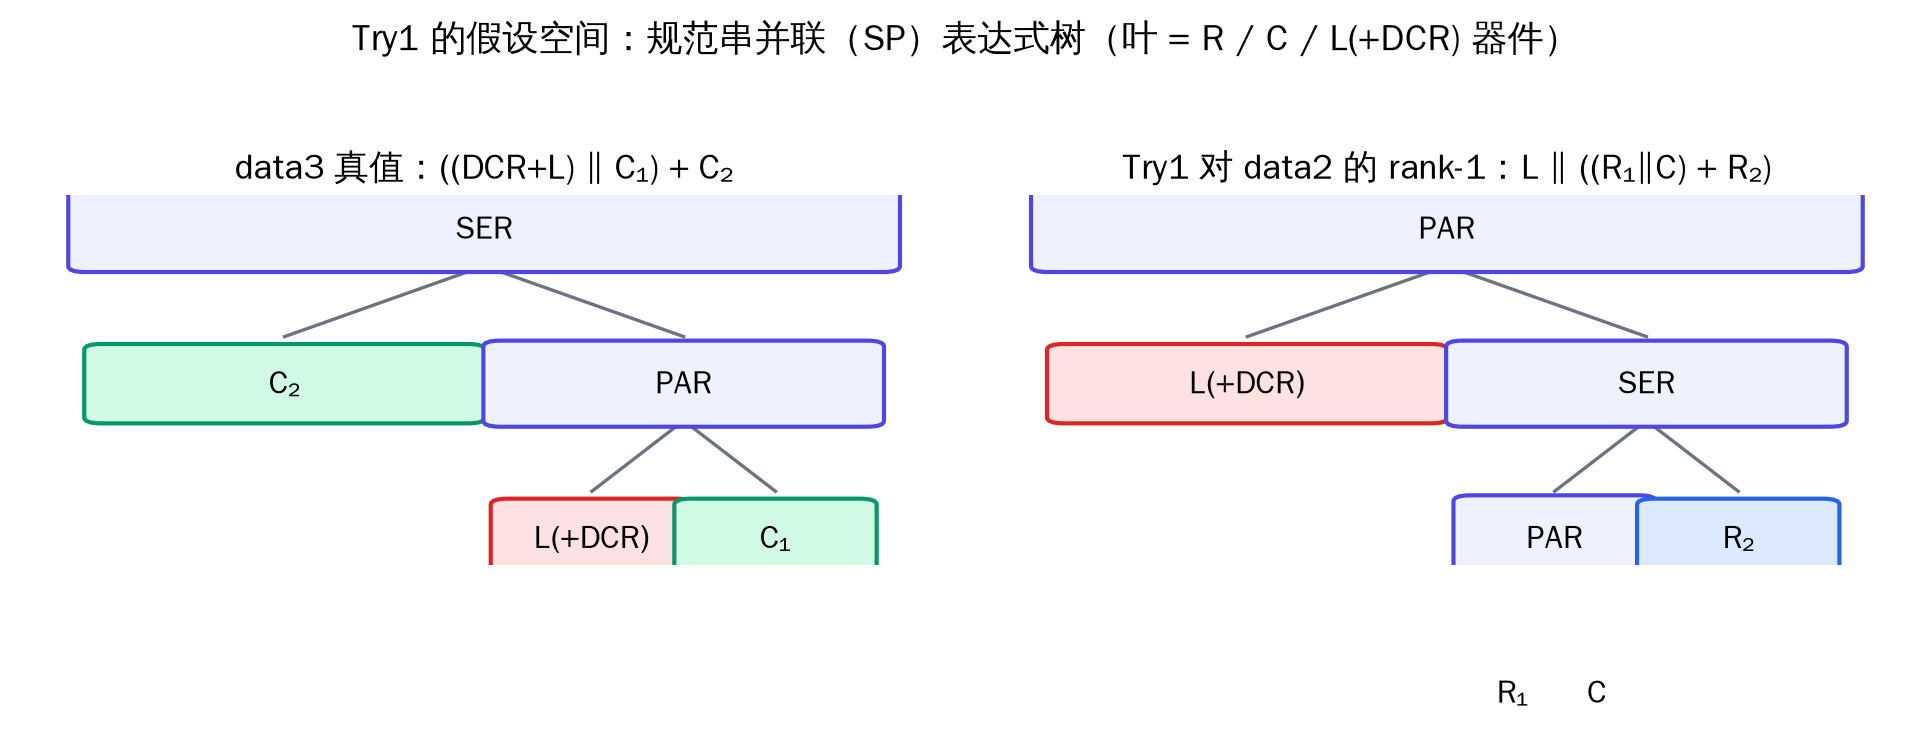
\includegraphics[width=\linewidth]{fig-sptree.png}\\
      \begin{beamercolorbox}[sep=4pt]{block body example}
        每棵树 expand 成图（SER 链生成内部节点）后，进入\textbf{同一个} $Z=b^{\mathsf T}Y^{-1}b$ 前向求值与共享拟合。
      \end{beamercolorbox}
    \end{column}
  \end{columns}
\end{frame}

% ------------------------------------------------ 13 try1 II
\begin{frame}{Try1（II）：有理拟合 $\to$ Foster 辅助候选}
  \begin{columns}
    \begin{column}{0.62\textwidth}
      \begin{block}{辅助路径：从数据直接综合候选电路}
        \begin{itemize}
          \item 尺度化（$s/\omega_0$、$Z/Z_0$）后做\textbf{实系数有理最小二乘}。
          \item 分母校正后用\textbf{特征值重定位}移动极点，再重拟合留数。
          \item 稳定极点 $\ne$ 无源性：\textbf{只接纳能显式综合为正值器件的 Foster 类}。
          \item 综合候选须过\textbf{共享前向模型一致性核对}，再进入公共精调与统一排序；综合失败只丢弃该候选，\textbf{绝不删除 SP 假设}。
        \end{itemize}
      \end{block}
      \begin{block}{两个被接纳的综合单元（归一化坐标，含尺度恢复）}
        {\small
        \[
          \frac{K}{s+a}=R\parallel C:\;\; R=\frac{K}{a},\;C=\frac{1}{K}
        \]
        \[
          \frac{Ks}{s^2+as+b}=R\parallel L\parallel C:\;\; R=\frac{K}{a},\;L=\frac{K}{b},\;C=\frac{1}{K}
        \]}
      \end{block}
    \end{column}
    \begin{column}{0.38\textwidth}
      \begin{block}{定位与边界}
        \begin{itemize}
          \item 这是一个\textbf{明确的 Foster 子族}，不是任意正实函数的通用综合（不含 Cauer/Brune）。
          \item SP 枚举完整 $\ne$ 连续内层全局最优，也不保证真实桥式结构在假设空间内。
          \item Strict 模式不做未证明安全的有限频带斜率删枝。
          \item 输出族 family = \texttt{NORMALIZED\_SP\_PLUS\_FOSTER}。
        \end{itemize}
      \end{block}
    \end{column}
  \end{columns}
\end{frame}

% ------------------------------------------------ 14 selection
\begin{frame}{模型选择：三层资格分层 + Top-K 行为等价类}
  \begin{columns}
    \begin{column}{0.46\textwidth}
      \begin{block}{候选三层（谁的 AICc 才算数）}
        {\scriptsize
        \begin{tabular}{@{}p{1.45cm}p{2.9cm}p{2.35cm}@{}}
          \toprule
          层 & 条件 & 排序依据\\
          \midrule
          primary & AICc 有效·收敛·非 robust·满秩·无触界 & AICc + 校准 $\Delta$\\
          provisional & 未收敛但其余正则 & 按 AICc 排序，无 $\Delta$\\
          diagnostic & AICc 无效 / robust / 秩亏 / 触界 & 原始 RSS 排在后\\
          \bottomrule
        \end{tabular}}
      \end{block}
      单个过参数候选失效只降级自己；无 primary 或 robust $\to$ \texttt{RSS\_DIAG\_FALLBACK}。
      \begin{block}{Top-K = 行为等价类}
        {\small
        \[
          \bigl|\hat Z_a(f_k)-\hat Z_b(f_k)\bigr|\le\varepsilon\max(\cdot)\quad\forall k
        \]}
        \vspace{-2ex}

        （$\varepsilon$ 默认 $10^{-6}$）同类只出代表元；等价是 \textbf{observed-grid} 数值等价，非符号恒等、非连续频带等价。
      \end{block}
    \end{column}
    \begin{column}{0.54\textwidth}
      \centering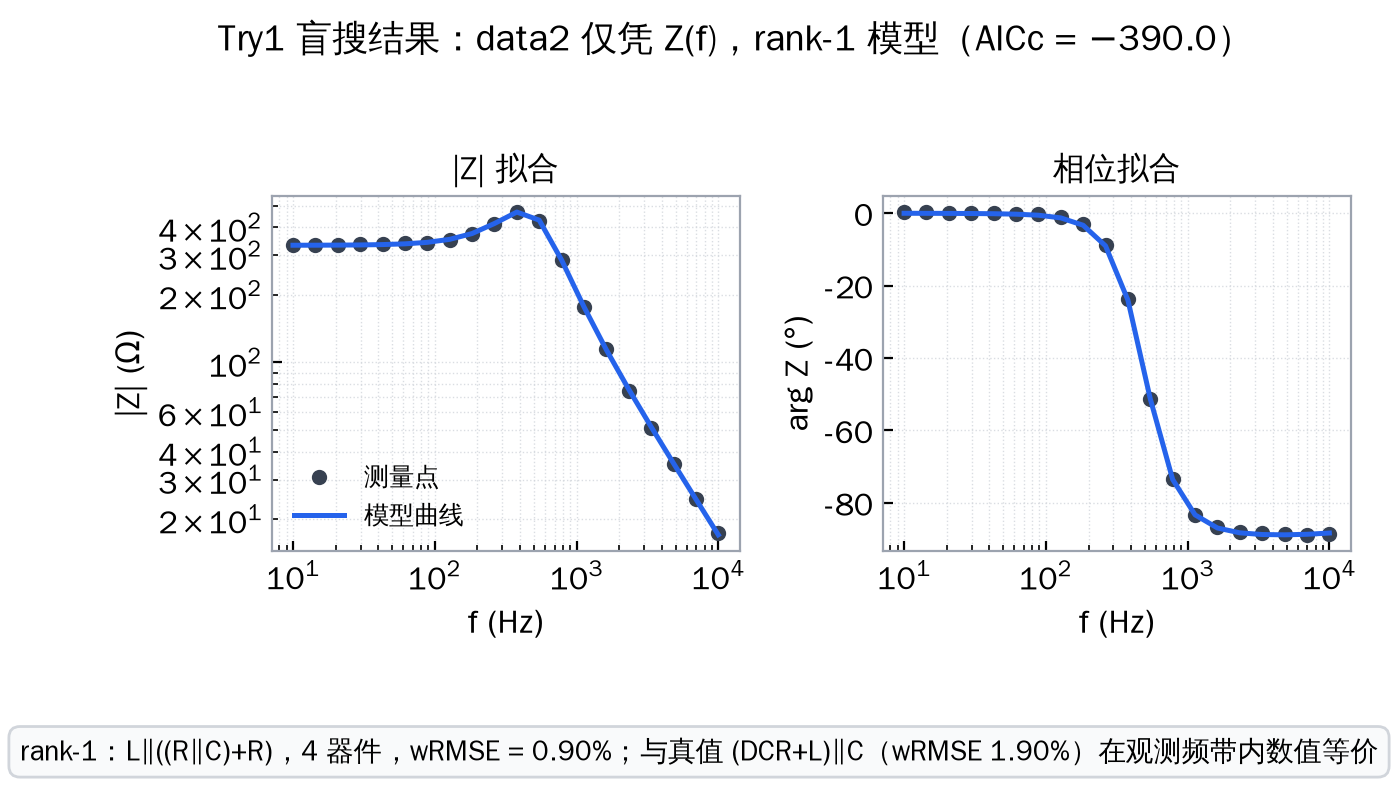
\includegraphics[width=0.88\linewidth]{try1-data2-2.png}\\[1pt]
      {\scriptsize
      \setlength{\tabcolsep}{3pt}
      \resizebox{\linewidth}{!}{%
      \begin{tabular}{@{}cccccc@{}}
        \toprule
        rank & 模型（data2 盲搜） & 器件 & wRMSE & AICc & $\Delta$\\
        \midrule
        1 & $L\parallel((R\parallel C){+}R')$ & 4 & 0.90\% & $-390.0$ & 0\\
        3 & $(L{+}DCR)\parallel C$ 微调 & 4 & 0.96\% & $-385.2$ & 4.8\\
        5 & $C\parallel L(+DCR)\parallel R$ & 3 & 1.18\% & $-371.4$ & 18.6\\
        \bottomrule
      \end{tabular}}}
    \end{column}
  \end{columns}
\end{frame}

% ------------------------------------------------ 15 results I
\begin{frame}{实测拟合效果 I：Try3 \textperiodcentered\ data2 = (DCR+L) $\parallel$ C}
  \begin{columns}
    \begin{column}{0.60\textwidth}
      \centering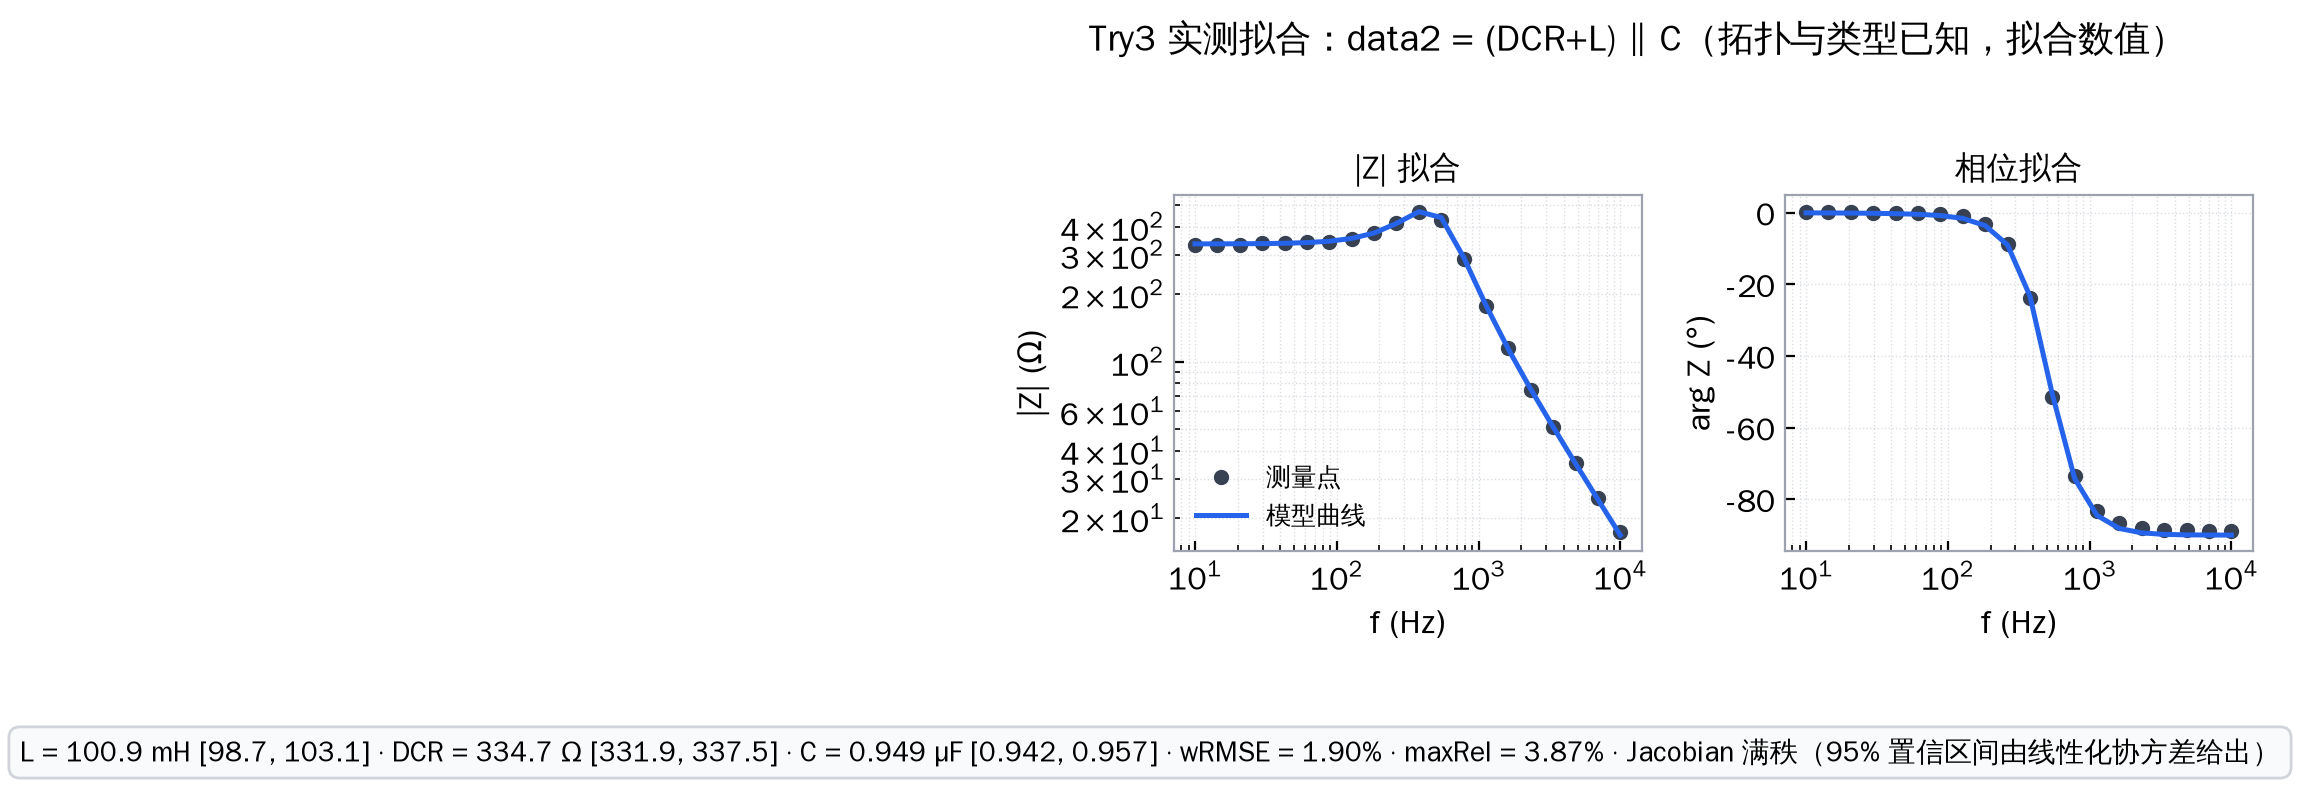
\includegraphics[width=\linewidth]{try3-data2-2.png}
    \end{column}
    \begin{column}{0.40\textwidth}
      \begin{block}{回收参数（20 点，3 自由参数）}
        {\scriptsize
        \begin{tabular}{@{}lccc@{}}
          \toprule
          参数 & 拟合值 & 95\% CI & 标称\\
          \midrule
          L & 100.9 mH & [98.7, 103.1] & 100 mH\\
          DCR & 334.7 Ω & [331.9, 337.5] & 345 Ω\\
          C & 0.949 µF & [0.942, 0.957] & 1 µF\\
          \bottomrule
        \end{tabular}}
      \end{block}
      \begin{block}{质量指标}
        wRMSE = \textbf{1.90\%}，maxRel = 3.87\%；Jacobian 满秩 $\to$ \textbf{IDENTIFIABLE\_LOCAL}；约 500 Hz 并联谐振（$Q\approx0.9$）被完整捕获。
      \end{block}
      \begin{beamercolorbox}[sep=4pt]{block body}
        回收值与标称的偏差来自元件容差（C 实际 $\approx$0.95 µF）——评价拟合应与独立复核的“回收真值”而非标称比较。
      \end{beamercolorbox}
    \end{column}
  \end{columns}
\end{frame}

% ------------------------------------------------ 16 results II
\begin{frame}{实测拟合效果 II：噪声数据与四组总表}
  \begin{columns}
    \begin{column}{0.60\textwidth}
      \centering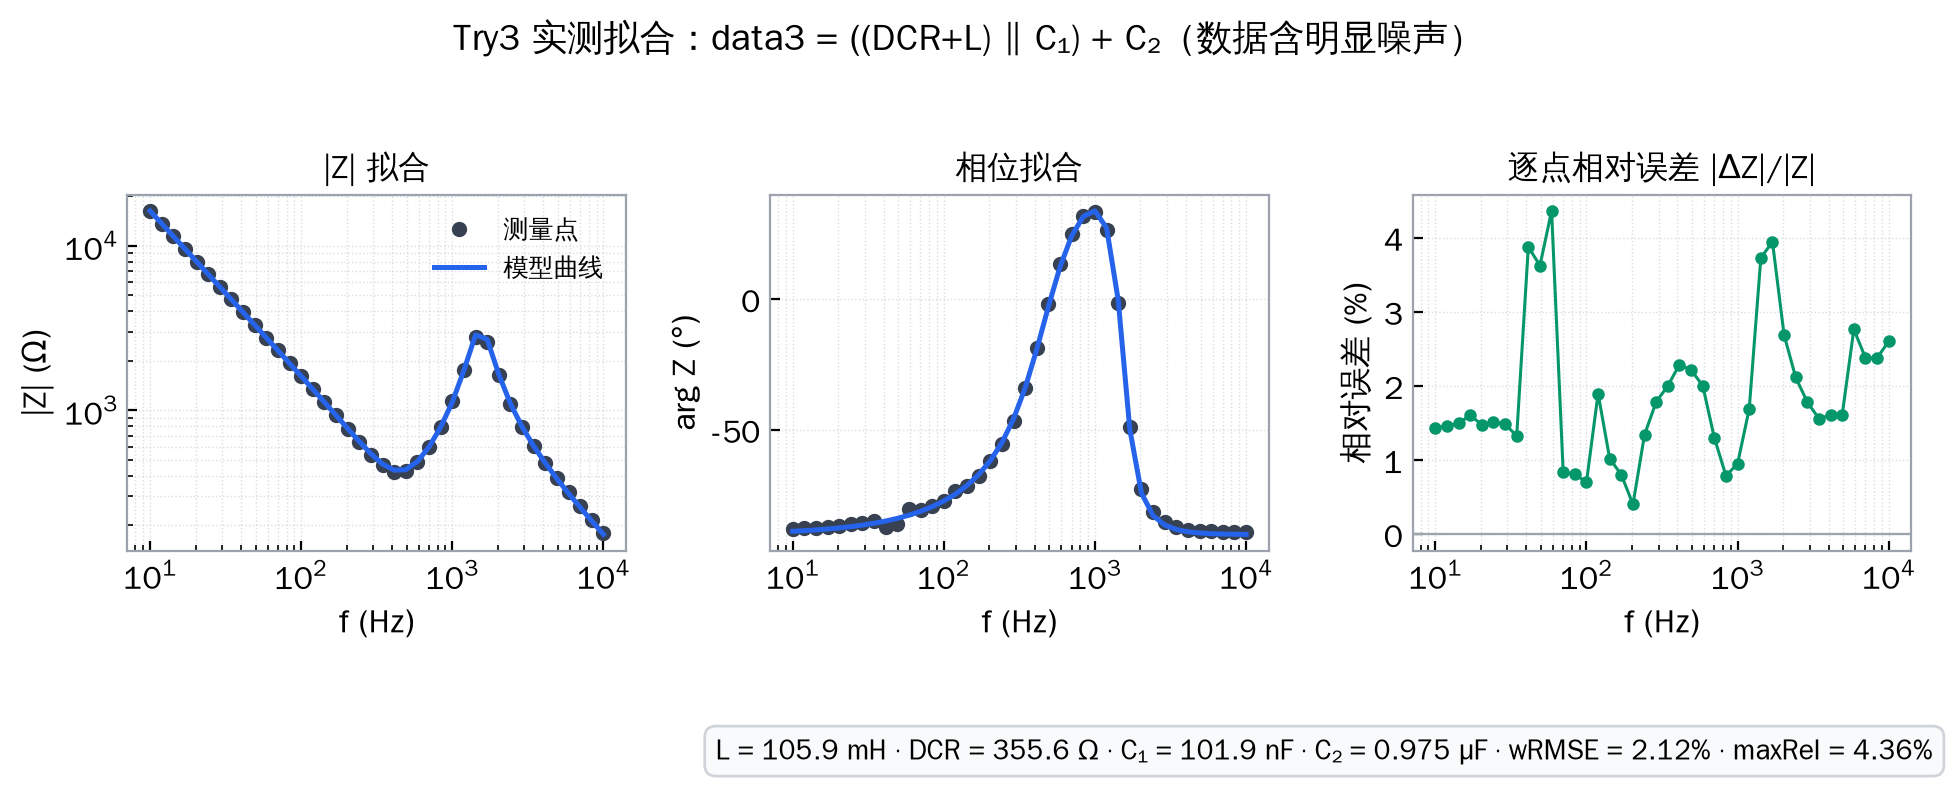
\includegraphics[width=\linewidth]{try3-data3-3.png}\\
      {\scriptsize data3（40 点，含明显噪声）：wRMSE 2.12\%，逐点相对误差基本在 $\pm4\%$ 内}
    \end{column}
    \begin{column}{0.40\textwidth}
      \begin{block}{四组实测 \textperiodcentered\ rank-1 wRMSE（\%）}
        {\scriptsize
        \begin{tabular}{@{}lcccc@{}}
          \toprule
          数据 & Try1 & Ex$^{*}$ & Tol$^{\dagger}$ & Try3\\
          \midrule
          data1 $R\parallel C$ & 0.53 & 2.34 & 0.92 & 0.92\\
          data2 $(r{+}L)\parallel C$ & 0.90 & 5.61 & 1.90 & 1.90\\
          data3 加串 $C_2$ & 1.47 & 6.36 & 2.12 & 2.12\\
          data4 串并槽路 & 0.50 & 5.26 & 0.50 & 0.50\\
          \bottomrule
        \end{tabular}\\[2pt]
        $^{*}$Try2 Exact（标称值，0 自由参数）\;$^{\dagger}\pm10\%$ 容差}
      \end{block}
      \begin{beamercolorbox}[sep=4pt]{block body example}
        随机基准 40 例（固定种子）：行为 pass@1 35/40，pass@8 39/40。Try1（盲搜）达到甚至优于带标称先验的 Try2——AICc 分层 + 多起点局部拟合在观测频带内足够锋利；Try2 Exact 的差距纯粹来自元件容差。
      \end{beamercolorbox}
    \end{column}
  \end{columns}
\end{frame}

% ------------------------------------------------ 17 boundaries
\begin{frame}{哪些结论不能宣称（以及为什么）}
  \begin{columns}
    \begin{column}{0.64\textwidth}
      \begin{alertblock}{诚实边界}
        \begin{itemize}
          \item \textbf{端口行为 $\ne$ 物理内部。}$R_1{+}R_2$ 与等值 R、$R{+}(R_d{+}sL)$ 与等值 L+DCR 永远不可区分；exactN 是等效模型器件数，不是 BOM 数。
          \item \textbf{行为等价是数值的、局部的。}observed-grid 等价只在观测频点成立。实测例：Try1 在 data4 的 rank-1 为 $R{+}(L\parallel(C{+}R'))$，与真值结构不同、wRMSE 同为 0.50\%。
          \item \textbf{局部最优无全局证书。}多起点只提高可信度，不证明连续参数全局最优；Try2.5/Tolerance/连续拟合一律 continuous\_global\_certified = false。
          \item \textbf{满秩 $\ne$ 唯一。}满列秩只支持局部可辨识；单点秩亏不证明全局参数族；weak 弹性度是经验阈值。
          \item \textbf{数值诊断不是误差界。}rcond / 后向误差是浮点可靠性诊断；AICc 在非线性、有界、系统误差场景只是近似。
        \end{itemize}
      \end{alertblock}
    \end{column}
    \begin{column}{0.36\textwidth}
      \begin{block}{成果如何如实呈现}
        \begin{itemize}
          \item Top-K 输出\textbf{行为等价类}代表元与成员数，而非“唯一电路”。
          \item 每个候选自带诊断（收敛、秩、边界、数值状态）。
          \item 枚举完成 / 预算耗尽 / 数值警告在运行级分开标记。
          \item 失败与部分结果显式暴露，不用哨兵值掩盖。
        \end{itemize}
      \end{block}
    \end{column}
  \end{columns}
\end{frame}

% ------------------------------------------------ 18 summary
\begin{frame}{总结：一条管线，三档先验}
  \begin{block}{统一管线（三个引擎共享同一个数学实现）}
    \centering\footnotesize
    测量 $Z(f_k)$ $\to$ 候选 $(G,\theta)$ $\to$ stamp 组装 $Y(s)$ $\to$ $Z_{\mathrm{calc}}=b^{\mathsf T}Y^{-1}b$\\[1pt]
    $\to$ 白化残差 $r_k$ $\to$ $J=\sum\|r_k\|^2$ $\to$ 搜索 / LM 优化 $\to$ 分层排序 Top-K + 诊断
  \end{block}
  \begin{columns}
    \begin{column}{0.48\textwidth}
      \begin{block}{三个关键公式}
        \[
          Z=b^{\mathsf T}Y^{-1}b,\qquad
          \frac{\partial Z}{\partial q_e}=-\frac{\partial y_e}{\partial q_e}(V_u-V_v)^2
        \]
        \[
          \mathrm{AICc}=n\log(J/n)+2k+\frac{2k(k+1)}{n-k-1}
        \]
      \end{block}
    \end{column}
    \begin{column}{0.52\textwidth}
      \begin{block}{三个引擎一句话}
        \begin{itemize}
          \item \textbf{Try1}：枚举规范 SP 树 + Foster 辅助——结构、类型、数值全要猜。
          \item \textbf{Try2}：器件已知，完整枚举非同构多重图——结构猜完直接比。
          \item \textbf{Try3}：结构已知，归约 + 解析灵敏度 LM——把数值钉到最优点并给出可辨识性诊断。
        \end{itemize}
      \end{block}
    \end{column}
  \end{columns}
  \begin{center}
    \begin{beamercolorbox}[center,sep=4pt]{block body example}
      \footnotesize 每猜出一个候选电路，判断方法永远一样：灌 1 A 电流 $\to$ 解 $Yv=b$ $\to$ $Z=V_1$ $\to$ 与测量比较。
    \end{beamercolorbox}
  \end{center}
\end{frame}

\end{document}
